\documentclass[11pt]{revtex4}
\usepackage[utf8x]{inputenc}
\usepackage{graphicx}
\usepackage{amssymb}
\usepackage{epstopdf}
\usepackage{mystyle}
\usepackage{amsmath}
\usepackage{bm}

\begin{document}

\title{Estimating quantum mechanical effects of atomic solids using quantum molecular dynamics with dissipation}
\author{Bing Gu}

\begin{abstract}
Atomic solids 
\end{abstract}

\maketitle

\section{Introduction}
Quantum molecular dynamics with dissipation, relevant to many processes in chemistry, physics, and biology, is a long-standing theoretical challenge. Dissipation describes interaction of the system with the bath, representing the environmental degrees of freedom. With few exceptions, the numerically exact simulations of such quantum processes occurring in condensed phase, have been performed, using path integral Monte Carlo methods for models consisting of a low-dimensional system coupled to a bath of harmonic oscillators.2,3 Inclusion of friction directly into the \se may be viewed as a simple way to mimic the effect of energy transfer from the system to the environment while limiting quantum dynamics calculations to the system degrees of freedom. Such picture is simplistic, yet it might be useful for some processes. For example, the quantum transition state theory of dissipative tunneling reproduces measurement of the H/D motion on Pt(111) surface with few adjustable parameters.

The force of friction, often taken for processes in condensed phase as linear in velocity of a particle, is most straightforwardly incorporated into equations of motion of a classical particle, characterized by position $x_t$ and momentum $p_t$, 
\be \frac{dp_t}{dt}=-\frac{dV(x)}{dx}-\gamma p_t |_{x=x_t}, ~\frac{dx_t}{dt}=\frac{p_t}{m}. \ee
The trajectory evolves under the influence of an external potential $V(\bm x)$, which is a function of the Cartesian coordinate, $\bm x$, parameter $\gamma$ denotes the friction coefficient.

\section{Formulation}
The friction term for the time-dependent \se (TDSE) can be incorporated into the de Broglie-Bohm formulation of TDSE. 
The friction term depends on the velocity of each quantum trajectory. The resulting TDSE is nonlinear; the time-dependent wavefunction conserves normalization, while the total energy of the wavefunction decreases with time to the zero-point energy value.
The new equations of motion with friction term for quantum trajectories in the Lagrangian frame of reference are as follows:

\begin{flalign} 
	\frac{dp}{dt} &= -\frac{\partial}{\partial x} (V+U)-\gamma p \label{eq:mom_fric} \\ 
	\frac{dx}{dt} &= -\frac{p}{m} 
\end{flalign}
Integrating Eq. (\ref{eq:mom_fric}) with respect to $x$, the evolution of $S(x,t)$ with friction becomes
\be -\frac{\pa S}{\pa t} = \frac{p^2}{2m} + V + U+ \gamma S + C(t). \label{eq:action_fric} \ee
The constant of integration $C(t)$ is defined in \ref{sophya2011}, 
%the overall phase of a wavefunction should not affect its evolution, including wavefunctions describing eigenstates. This requirement is satisfied by the choice, 
\be C(t) = -\bra S(x,t) \ket. \ee
Together with continuity equation unchanged by friction, the conventional TDSE with friction becomes
\be \imath \hbar \frac{\pa }{\pa t}\psi(x,t) = \hat{H}\psi(x,t) + \gamma (S(x,t) - \bra S(x,t) \ket)\psi(x,t). \ee

%******************************************************************************************************
\subsection{Global linear approximation to nonclassical momentum} \label{sec:lqf}
Quantum potential, $U$, is responsible for all \qm effects, such as zero-point energy and quantum-mechanical tunneling. The classical limit is defined as $U \rightarrow 0$. 
%We use the QT formalism as a well-defined semiclassical propagation method by making a single approximation to the quantum potential. 
A simple approximation can be made to compute quantum potential ``fast'' and accurate. Details about the linearized quantum force (LQF) methodology is described in \cite{garashchuk2004}.
We briefly review this method here.
The essential idea is to get approximated quantum potential from the global linear least-squares fitting of the nonclassical component of the momentum operator \cite{garashchuk2004}, 
\be r_\alpha(\bm{x},t) = \frac{\grad_\alpha A(\bm x,t)}{A(\bm x,t)}\approx \tilde{r}_\alpha(\bm x,t)\label{eq:r}\ee at each time step in small basis $\bm{f}(\bm x)$, which is analytically determined. We use greek letters $\alpha, \beta, \dots$ to label an arbitrary degree of freedom. 
\be U \approx \sum_\alpha \frac {- \hbar^2}{2m} (\tilde{r}_\alpha \cdot \tilde{r}_\alpha + \grad_\alpha \tilde{r}_\alpha). \label{eq:rfit} \ee
The least-squares fitting \cite{nurec2} minimizes $\sum_\alpha \bra (r_\alpha -\tilde{r}_\alpha)^2\ket$, where  $\tilde{r}_\alpha$ is 
represented in a linear basis $f(\bm x)$

For a multi-dimensional system, $\bm f(\bm x)$ can be arranged as a vector  $(1,x_1,x_2,\cdots)$, so the approximate nonclassical momentum component is  expressed as 
\be \tilde{r}={\bf C}\bm{f}, \ee
where $\bf C$ is a matrix of coefficients, which solves the matrix equation  
\be 2{\bf SC} + {\bf B}=0  \label{eq:mateq}. \ee 
The matrices are defined by the  outer product of vectors  
\be {\bf S}=\bra \bm{f} \otimes \bm{f}\ket,~ {\bf B}= \bra {\nabla} \otimes \bm{f} \ket^T \label{eq:mateq2}\ee
%which, when expanded, are
%\begin{flalign} \textbf{\bf{S}} = 
%\left( \begin{array}{cccc}
%	\bra 1 \ket & \bra x \ket & \bra y \ket \\
%	\bra x \ket & \bra x^2 \ket & \bra xy \ket \\
%	\bra y \ket & \bra xy \ket & \bra y^2 \ket  \\
%         \end{array}\right), ~~~
%\textbf{\bf{B}} = 
%\left( \begin{array}{ccc}
%	\bra 0 \ket & \bra 0 \ket  \\
%	\bra 1 \ket & \bra 0 \ket  \\
%	\bra 0 \ket & \bra 1 \ket  \\
%	     \end{array} \right)
%          \label{eq:mfit} \end{flalign}

The approximate quantum potential defined by Eqs. (\ref{eq:rfit}-\ref{eq:mateq2}) is simply a quadratic 
function of $\bm{x}$ yielding a linear quantum force (LQF) for every trajectory.  This approximation rigorously 
conserves energy and is exact for Gaussian wavepackets, but does not presume that $\psi(\bm{x},t)$ is necessarily a Gaussian wavefunction.  
%(Some other methods about approximations of quantum potential can be found in  Refs\cite{goldfarb2006,wyatt2000,gindensperger2000,kendrick2003,lopreore1999,trahan2003}.)
This simple approximation gives basic QM effects, such as wavepacket bifurcation, moderate tunneling and
zero-point energy. \cite{garashchuk_rcc}

While studying quantum dissipation, theoretically, the expectation value of energy will decay to the ground state,  which means the quantum force, $\grad U(\bm x,t)$, will cancel the classical force so that there is no net force for quantum trajectories. The challenge here is that for an anharmonic system, 
%$V(x) = \frac{x^2}{2}+\lambda x^4$, 
the linear quantum force does not have the corresponding high order term to balance classical force, which means the trajectories will never stop. With a small friction constant, the quantum trajectories will wiggle around equilibrium position and finally become localized.

\begin{figure}
	\includegraphics[width=0.8\textwidth]{figs/traj} \label{fig:lqf}
	\caption{Quantum trajectories for one-dimensional anharmonic potential, $V(x) = \frac{x^2}{2}+0.1x^4$, LQF is applied, $\alpha_0$ = 1, $\gamma$ = 0.05}
\end{figure}    

To fix this problem, a modification is proposed to account for anharmonicity. 
%To avoid this problem, one possible solution is to add more flexibility to the formula of quantum force. A straightforward method is to increase the basis size for the approximations of non-classical momentum. 


%\section{Eulerian frame of reference}
%
%There is an alternative frame of reference that can be used in the propagation of trajectories, which is the so called Eulerian frame. The equations of motion can be obtained through, the relationship of the rate of change for quantities in these two frame of references can be expressed in the following equation
%\be \frac{d}{dt} = \frac{\partial}{\partial t} + v \cdot \grad. \ee
%\be \frac{d}{dt} = \frac{\pa}{\pa t} + \sum_\alpha m^{-1}_\alpha\grad_\alpha S\grad_\alpha \ee
%Substitute this equation into the equations of motion in Lagrangian frame of reference, we can obtain 
%\begin{flalign}
%	\frac{\partial p}{\partial t} &= -\frac{p\grad p}{m}-\grad(V+U)-\gamma p. \label{eq:mom_fric} \\ 
%	\frac{\partial x}{\partial t} &= 0 \\   
%\end{flalign}
 
\section{Potential energy and force}
A pre-calculated potential describing the interaction of two helium atoms $V(r^2)$ is used to compute the potential for the whole system. The position vector $\vec{r}_{ij}$ between two helium atoms is defined as:
\be \vec{r}_{ij} = -d\vec{r}_i + \vec{d}_{ij} + d\vec{r}_j, \ee
where $d\vec{r}_i,~d\vec{r}_j$ are displacement vectors for atom $i$ and $j$,
\be d\vec{r}_i = \frac{dx_i}{|dr_i|}\vec{x} +  \frac{dy_i}{|dr_i|}\vec{y} + \frac{dz_i}{|dr_i|}\vec{z}. \ee 
 
The two-body potential is computed over a grid of the square of the distance between two atoms, the classical force over each DOF is computed as 
\be \frac{\partial V}{\partial dx_i} = \frac{\partial V}{\partial r_{ij}^2}\frac{\partial r^2_{ij}}{\partial dx_i}, \ee
\be r^2_{ij} = (-dx_i+x_{ij}+dx_j)^2+(-dy_i+y_{ij}+dy_j)^2+(-dz_i+z_{ij}+dz_j)^2, \ee 
\be \frac{\partial r^2_{ij}}{\partial dx_i} = 2(-dx_i+x_{ij}+dx_j). \ee 
%Finally, we get 
\be \frac{\partial V}{\partial dx_i} =  2(-dx_i+x_{ij}+dx_j) \frac{\partial V}{\partial r_{ij}^2} \ee 

\section{Long-range interactions correction}
Long-range interactions are calculated in the same way as for the short-range interactions. The long-range interaction for each atom is approximated by a polynomial $P_{N_b}(x,y,z)$ on the basis of,   
\be \bm{b} = \{1,x,y,z,x^2,y^2,z^2,xy,yz,xz \}^T, \ee
\be P_{N_b}(x,y,z) = \bm{b}^T\bm{c} \ee. 
We set up a three-dimensional grid of the displacements of atom on space and for each point $(x_i,y_i,z_i)$, we obtain the value of the long-range interaction $V_{l}(x_i,y_i,z_i)$ which is convergent to the number of atoms being used for the computation. Finally, we will get $N_p = N_x \times N_y \times N_z$ values and use these values to obtain the coefficients 
\be \bm{c} = \{ c_1,c_2,...c_{N_b} \}^T \ee 
before the each basis term. $N_b$ is the number of basis terms, which in this case is $10$.
The coefficients can be obtained by solving the matrix equation
\be {\bf M}\bm{c} = \bm{V_l}, \ee
where $\bf{M}$ is an $N_p \times N_b$ matrix, for each line, the elements are 
\be {\bf M}(i,j=1,\dots,N_b) = \{ 1,x_i,y_i,z_i,x_i^2,y_i^2,z_i^2,x_iy_i,y_iz_i,x_iz_i \}. \ee
and $\bm V_l$ is the vector of the interaction values at all points, 
\be \bm{V_l}(i) = V_l(x_i,y_i,z_i) \label{eq:mat}. \ee 
Since it is an overdetermined system, the matrix equation is solved under Least-Squares algorithm. 
%Since ${\bf M}$ is a huge matrix, to make it easier to solve, we times ${\bf M}^T$ for both sides of Eq. (\ref{eq:mat}), then we get 
%\be {\bf M}^T{\bf M}\bm{c} = {\bf M}^T \bm{V_l}, \ee
%where ${\bf M}^T{\bf M}$ is a $N_b \times N_b$ matrix, we can call subroutine $DPOSV$ from $LAPACK$ to solve the new matrix equation.  
    
\section{Equations of motion for ($x,p,r$)}

Starting from continuity equation
\be \frac{\partial \rho(\bm x,t)}{\partial t} + \bm \grad \left(\rho(\bm x,t)\frac{\bm p}{m}\right) = 0 \ee
substitute $ \rho = A^2 $ into the continuity equation, we will obtain
\be 2A\partial_tA + \sum_\alpha \left( 2A\grad_\alpha A m^{-1}_\alpha p_\alpha + A^2 \grad_\alpha p_\alpha  m_\alpha^{-1} \right) = 0 \ee
divide by $2A^2$, 
\be \pa_t \log A = -\sum_\alpha \left( {\grad_\alpha \log A p_\alpha}{m^{-1}_\alpha}  +  \frac{\grad_\alpha p_\alpha}{2m_\alpha} \right) \ee
use partial derivative operator $\grad_\alpha$ operate on both sides of the last equation and notice $r_\alpha = \grad_\alpha \log A$, we will get 
\be  \dot{r}_\alpha = -\left( \sum_\beta \frac{\grad_\alpha p_\beta}{m_\beta}r_\beta +\sum_\beta \frac{\grad_\alpha \grad_\beta p_\beta}{2m_\beta}\right)  \ee

Then in Lagrangian frame of reference, the exact equations of motion for ($x,p,r$) will be 
\begin{flalign}
  \dot{x}_\alpha &= \frac{p_\alpha}{m_\alpha} \\
  \dot{p}_\alpha &= -\grad_\alpha \left( V(\bm x)+U(\bm x,t) \right) \\
  \dot{r}_\alpha &= -\left( \sum_\beta \frac{\grad_\alpha p_\beta}{m_\beta}r_\beta +\sum_\beta \frac{\grad_\alpha \grad_\beta p_\beta}{2m_\beta}\right)  
\end{flalign}
where 
\be \tilde(U(x,t) = \sum_\alpha (\tilde{r}(x,t)^2_\alpha + \grad_\alpha \tilde{r}) \ee
$\bm{x},\bm{p}$ are position and momentum vectors with dimensionality of $3N$, $N$ is the number of particles. 
%To better illustrate the equations, we take a 2 dimenisonal system for example,

Instead of applying linear basis, qubic basis $(1,x,x^2,x^3)$ is used to approximate non-classical momentum $r$, as well as classical momentum $p$. 
By doing this, we kind of add some freedom to the formula of quantum force but constraint to the motion of trajectories. 
The new equations of motion with fitted terms in Lagragian frame of reference, $\tilde{p},\tilde(r)$ will be 

\begin{flalign}
  \dot{x}_\alpha &= \frac{\tilde{p}_\alpha}{m_\alpha} \\
  \dot{p}_\alpha &= -\grad_\alpha \left( V(\bm x)+\tilde{U}(\bm x,t) -\gamma p_\alpha \right) \\
  \dot{r}_\alpha &= -\left( \sum_\beta \frac{\grad_\alpha \tilde{p}_\beta}{m_\beta}\tilde{r}_\beta +\sum_\beta \frac{\grad_\alpha \grad_\beta \tilde{p}_\beta}{2m_\beta}\right)  
\end{flalign}


%\subsection{One dimensional model}
%Consider an harmonic oscilator with an anharmonic quatic term 
%\be V(x) = \frac{1}{2} (x^2+x^4) \ee 
%Choose initial wavefunction as a Gaussian 
%\be \psi(x,0) = \sqrt[4]{\frac{2\alpha}{\pi}}\exp \left(-\alpha (x-x0)^2+\im p(x-x0)\right) \ee
%Parameters are chosen as $x_0 = 0, ~p = 0$. 
%
%\begin{figure}[htbp]
%\begin{center}
%\includegraphics[width=1\textwidth]{/Users/bing/Labwork/friction/rp2/energy.pdf}
%\caption{Energy  components with $\gamma = 6$}
%\label{fig:energy_1d}
%\end{center}
%\end{figure}
%
%\begin{figure}[htbp]
%\begin{center}
%\includegraphics[width=1\textwidth]{/Users/bing/Labwork/friction/rp2/traj.pdf}
%\caption{Propagation of trajectories  with $\gamma = 6$}
%\label{fig:traj_1d}
%\end{center}
%\end{figure}

\section{Modification of approximation for quantum force}
Fitting with larger basis can cause a dramatic  increase in computational cost. The size of the basis $x_ix_j$ will be $1+3N_{atom}+\frac{3N_{atom}(3N_{atom}-1)}{2}$ if we want to include cubic basis for each DoF and all the linear coupling terms. To save computational efforts, the least-square fitting procedure is decomposed into two steps after we realize for each DoF, there are some terms that are of little contribution to the fitting, which means the coefficients before these terms remains a small number close to 0.

 \begin{itemize}
 \item The first step is to apply a linear basis $(1,x,y,\dots)$ to do least-square fitting of $(\bm p, \bm r)$ to minimize $\sum_\alpha || (r_\alpha(x,t) - \tilde(r)_\alpha(x,t) ||_2$ and $\sum_\alpha || (p_\alpha(x,t) - \tilde(p)_\alpha(x,t) ||_2$,  the fitted terms can be expressed by

 \item The second step is to fit the remainder with a cubic basis for each degree of freedom, $(1,x_\alpha,x_\alpha^2,x_\alpha^3)$. The other terms in the basis include linear terms of other DoFs, $(x_\beta, \beta = 1..N_c)$, and linear coupling terms $(x_\alpha x_\beta)$. $N_c$ is the number of the coupling DoFs that will be included. 
%The full basis for DoF $\alpha$ will be 
 %\be \bm {f}_\alpha = (1,x_\alpha,x_\alpha^2,x_\alpha^3, x_{\beta, \beta = 1..N_c}, x_\alpha x_{\beta, \beta=1..N_c) \ee.  
 \end{itemize}


\subsection{Two-dimensional model}
We design a two-dimensional potential, which represent two linearly coupled anharmonic vibrational mode. 
\be V(x,y) = \frac{1}{2} (x^2+x^4) + \frac{1}{2} (y^2+y^4)+\epsilon xy  \ee 
$\epsilon$ is a parameter that can be used to control the coupling between two degrees of freedom.
 
\begin{figure}[htbp]
\includegraphics[width=0.8\textwidth]{/Users/bing/Labwork/friction/2d8/energy.pdf}
\caption{Energy components with $\gamma = 6$}
\label{fig:traj_1d}
\end{figure}

%In Eulerian frame of reference, the the equations of motion for ($p,r$) will be similar 
%\begin{flalign}
%  \frac{\partial}{\partial p} &= -\frac{p\grad p}{m}-\grad(V+U) \\ 
%  \frac{\partial}{\partial r} &= -\frac{p\grad r}{m}-\left(\frac{\grad p}{m}r+\frac{\grad^2 p}{2m}\right) 
%\end{flalign}
%\begin{figure}

\section{Numerical Implementation}
The implemented code is paralleled by \textit{Message Passing Interface} (MPI), Fig \cite{fig:scale} shows the scaling of the computational cost for different number of processors.
\begin{figure}
	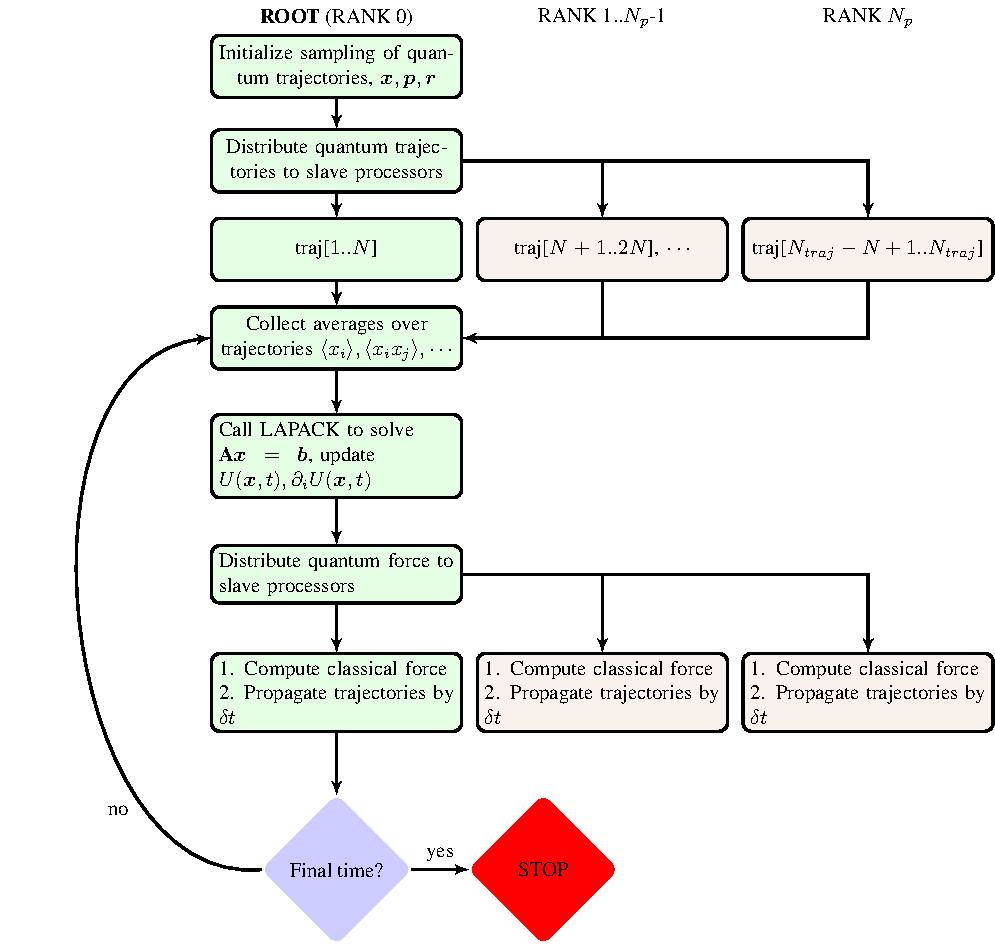
\includegraphics[width=0.8\textwidth]{flowchart/qtm_mpi}
	\caption{Flowchart of parallelization, quantum trajectories are distributed among processors such that the computing of classical force is paralleled} 
\end{figure}

\section{Results}

\section{Dynamic properties}
\begin{itemize}
  \item using electronic structure (for example, DFT, DFTB may not work)  theory to get potential energy, to see if many-body interactions are important 
  \item  tbd
\end{itemize}

\section{Radial distribution function}
To have a theoretical measure of the inter-atom distance distribution at ground state for atomic solids accounting for quantum effects, it seems appropriate to define a radial distribution function 
\begin{align}
 g(r) & = \frac{1}{4\pi \rho N r^2}\frac{\bra \psi_0(\bm r_1, \cdots, \bm r_N)  | \sum_{i,j \neq i}^N \delta(r - |r_{ij}|) | \psi_0(\bm r_1, \cdots, \bm r_N) \ket}{\bra \psi_0(\bm r_1, \cdots, \bm r_N ) | \psi_0(\bm r_1, \cdots, \bm r_N) \ket} \\ 
	& =   \frac{1}{4\pi \rho N r^2}\sum_{i,j < i}^N \frac{\bra \psi_0(\bm r_1, \cdots, \bm r_N)  | \delta(r - |r_{ij}|) | \psi_0(\bm r_1, \cdots, \bm r_N) \ket}{\bra \psi_0(\bm r_1, \cdots, \bm r_N ) | \psi_0(\bm r_1, \cdots, \bm r_N) \ket}
\end{align}
for wavefunction with exchange symmetry, i.e. particles are indistinguishable 
\begin{align}
 g(r) & = \frac{N}{\rho}\frac{\bra \delta(r - |r_{12}|) \ket}{4\pi r^2}  \\ 
% \frac{\bra \psi_0(\bm r_1, \cdots, \bm r_N)  | \delta(r - |r_{12}|) | \psi_0(\bm r_1, \cdots, \bm r_N) \ket}{\bra \psi_0(\bm r_1, \cdots, \bm r_N ) | \psi_0(\bm r_1, \cdots, \bm r_N) \ket} \\  
	&  = \frac{N}{4\pi \rho r^2} \int d\bm r_1 d\bm r_2 \delta(r - |\bm r_{12}|)\rho(\bm r_1,\bm r_2) 
\end{align}
where $\rho(\bm r_1, \bm r_2)$ is the joint probability. 
\be \rho(\bm r_1, \bm r_2) = \int d\bm r_3\cdots d\bm r_N~ \rho(\bm r_1,\cdots,\bm r_N) \ee 
We would like to see if the form would give right solution at two limiting cases. 

The first limiting case is a perfect solid, every atom has a fixed position in space, $\bm R_i$.
\be g(r) = \sum_{i,j \neq i} \delta(r-|\bm R_{ij}|) \ee 
the pair distribution function will be peaks at all the possible distance, which is what we expect to see. 

Another case is non-interacting limit and the ground state density can be approximated with a uniform distribution $\rho(\bm r_1, \bm r_2) = (\frac{1}{V})^2$, the system should behave like ideal gas.  
The PDF will be  
\begin{flalign}  
g(r) & = \frac{N}{\rho}  (\frac{1}{V})^2 \int d\bm r_1 d\bm r_2 \frac{\delta(r - | \bm r_{12}|)}{4\pi r^2} \\ 
 	& = \frac{N}{\rho V} \\ 
	& = 1 ~( ideal~gas) \\   
\end{flalign}

System in reality should be in the intermediate of this two limiting cases, for small vibrations in the equilibrium position ($|\delta \bm r| << |\bm r|$), a spreading of the infinity peak is likely to show up. 
For numerical difficulty, we would use a Gaussian function to replace the $\delta$ function, or draw a histogram for different intervals, by counting trajectories with $r_{12}$ fitting that range.  
\be \delta(x) = \lim_{\alpha \rightarrow \infty} \sqrt{\frac{2\alpha}{\pi}} e^{-\alpha x^2} \ee   
 

try new density $\rho = 0.005231~a. u.$ to compute pair distribution function.   
change the long-range potential fitting to fit the density. 



\end{document}
